\begin{figure}[htbp]
\centering

\tikzstyle{input}=[rectangle,
                                    thick,
                                    minimum size=0.25cm,
                                    draw=gray!20,
                                    fill=gray!20]

\tikzstyle{rnn}=[rectangle,
                                    thick,
                                    minimum height=0.5cm,
                                    minimum width=1cm,
                                    draw=blue!80,
                                    draw=blue!80,
                                    fill=blue!20]

\tikzstyle{encoder}=[rectangle,
                                    thick,
                                    minimum height=0.5cm,
                                    minimum width=1cm,
                                    draw=yellow!80,
                                    fill=yellow!20]

\tikzstyle{empty}=[rectangle,
                                    thick,
                                    minimum height=0.5cm,
                                    minimum width=1cm,
                                    draw=white!0,
                                    fill=white!0]

\tikzstyle{output}=[rectangle,
                                    thick,
                                    minimum size=0.25cm,
                                    draw=gray!20,
                                    fill=gray!20]

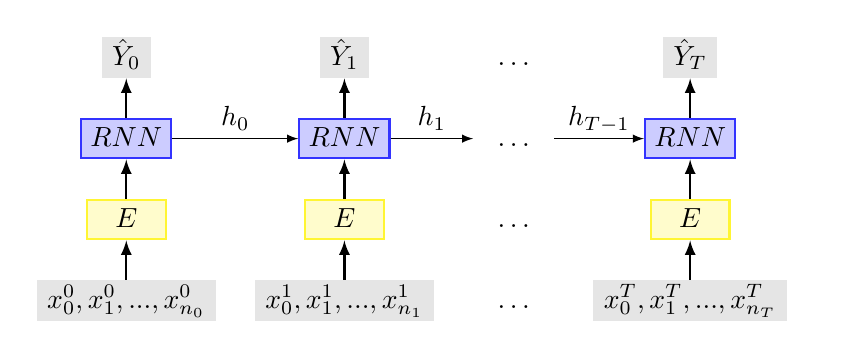
\begin{tikzpicture}[>=latex,text height=1.5ex,text depth=0.25ex]
    % "text height" and "text depth" are required to vertically
    % align the labels with and without indices.
  
  % The various elements are conveniently placed using a matrix:
  \matrix[row sep=0.5cm,column sep=0.5cm] {

	% First line: Output labels
	\node (Y_0) [output]{$\hat{Y}_0$};&
	\node (Y_1) [output]{$\hat{Y}_1$};&
  \node (dots1) [empty] {$\dots$};  &
	\node (Y_T) [output]{$\hat{Y}_T$};&
	\\
	% Second line: RNNs
	\node (RNN_0) [rnn]{$RNN$};&
	\node (RNN_1) [rnn]{$RNN$};&
  \node (dots2) [empty] {$\dots$};  &
	\node (RNN_T) [rnn]{$RNN$};&
	\\
	% Third line: Linear layers
	\node (Encoder_0) [encoder]{$E$};&
	\node (Encoder_1) [encoder]{$E$};&
  \node (dots3) [empty] {$\dots$};  &
	\node (Encoder_T) [encoder]{$E$};&
	\\
	% Fourth line: Linear layers
	\node (Input_0) [input]{$x^0_{0},x^0_{1},...,x^0_{n_0}$};&
	\node (Input_1) [input]{$x^1_{0},x^1_{1},...,x^1_{n_1}$};&
  \node (dots4) [empty] {$\dots$};  &
	\node (Input_T) [input]{$x^T_{0},x^T_{1},...,x^T_{n_T}$};&
        \\
    };
    
    % The diagram elements are now connected through arrows:
    \path[->]
        (Input_0) edge[thick]  (Encoder_0)	
        (Input_1) edge[thick] (Encoder_1)	
        (Input_T) edge[thick] (Encoder_T)	

        (Encoder_0) edge[thick] node[right] {} (RNN_0)	
        (Encoder_1) edge[thick] node[right] {} (RNN_1)	
        (Encoder_T) edge[thick] node[right] {} (RNN_T)	

        (RNN_0) edge[thick] (Y_0)	
        (RNN_1) edge[thick] (Y_1)	
        (RNN_T) edge[thick] (Y_T)	

        (RNN_0) edge node[above] {$h_0$} (RNN_1)
        (RNN_1) edge node[above] {$h_1$} (dots2)
        (dots2) edge node[above] {$h_{T-1}$} (RNN_T)
        ;
    
\end{tikzpicture}

\captionsetup{format=plain}
\caption{Simple neural DAR model. Utterance $t$ with tokens $x_0,...,x_{n_t}$ is encoded by $E$, then passed as input to the RNN. The RNN's hidden state, $h{t-1}$ models the discourse context at utterance $t$. The output layer of the RNN predicts the dialogue act, $\hat{Y}_t$.}
\label{fig:architecture}
\end{figure}
